% Options for packages loaded elsewhere
\PassOptionsToPackage{unicode}{hyperref}
\PassOptionsToPackage{hyphens}{url}
\PassOptionsToPackage{dvipsnames,svgnames,x11names}{xcolor}
%
\documentclass[
  letterpaper,
  DIV=11,
  numbers=noendperiod]{scrartcl}

\usepackage{amsmath,amssymb}
\usepackage{lmodern}
\usepackage{iftex}
\ifPDFTeX
  \usepackage[T1]{fontenc}
  \usepackage[utf8]{inputenc}
  \usepackage{textcomp} % provide euro and other symbols
\else % if luatex or xetex
  \usepackage{unicode-math}
  \defaultfontfeatures{Scale=MatchLowercase}
  \defaultfontfeatures[\rmfamily]{Ligatures=TeX,Scale=1}
\fi
% Use upquote if available, for straight quotes in verbatim environments
\IfFileExists{upquote.sty}{\usepackage{upquote}}{}
\IfFileExists{microtype.sty}{% use microtype if available
  \usepackage[]{microtype}
  \UseMicrotypeSet[protrusion]{basicmath} % disable protrusion for tt fonts
}{}
\makeatletter
\@ifundefined{KOMAClassName}{% if non-KOMA class
  \IfFileExists{parskip.sty}{%
    \usepackage{parskip}
  }{% else
    \setlength{\parindent}{0pt}
    \setlength{\parskip}{6pt plus 2pt minus 1pt}}
}{% if KOMA class
  \KOMAoptions{parskip=half}}
\makeatother
\usepackage{xcolor}
\setlength{\emergencystretch}{3em} % prevent overfull lines
\setcounter{secnumdepth}{-\maxdimen} % remove section numbering
% Make \paragraph and \subparagraph free-standing
\ifx\paragraph\undefined\else
  \let\oldparagraph\paragraph
  \renewcommand{\paragraph}[1]{\oldparagraph{#1}\mbox{}}
\fi
\ifx\subparagraph\undefined\else
  \let\oldsubparagraph\subparagraph
  \renewcommand{\subparagraph}[1]{\oldsubparagraph{#1}\mbox{}}
\fi

\usepackage{color}
\usepackage{fancyvrb}
\newcommand{\VerbBar}{|}
\newcommand{\VERB}{\Verb[commandchars=\\\{\}]}
\DefineVerbatimEnvironment{Highlighting}{Verbatim}{commandchars=\\\{\}}
% Add ',fontsize=\small' for more characters per line
\usepackage{framed}
\definecolor{shadecolor}{RGB}{241,243,245}
\newenvironment{Shaded}{\begin{snugshade}}{\end{snugshade}}
\newcommand{\AlertTok}[1]{\textcolor[rgb]{0.68,0.00,0.00}{#1}}
\newcommand{\AnnotationTok}[1]{\textcolor[rgb]{0.37,0.37,0.37}{#1}}
\newcommand{\AttributeTok}[1]{\textcolor[rgb]{0.40,0.45,0.13}{#1}}
\newcommand{\BaseNTok}[1]{\textcolor[rgb]{0.68,0.00,0.00}{#1}}
\newcommand{\BuiltInTok}[1]{\textcolor[rgb]{0.00,0.23,0.31}{#1}}
\newcommand{\CharTok}[1]{\textcolor[rgb]{0.13,0.47,0.30}{#1}}
\newcommand{\CommentTok}[1]{\textcolor[rgb]{0.37,0.37,0.37}{#1}}
\newcommand{\CommentVarTok}[1]{\textcolor[rgb]{0.37,0.37,0.37}{\textit{#1}}}
\newcommand{\ConstantTok}[1]{\textcolor[rgb]{0.56,0.35,0.01}{#1}}
\newcommand{\ControlFlowTok}[1]{\textcolor[rgb]{0.00,0.23,0.31}{#1}}
\newcommand{\DataTypeTok}[1]{\textcolor[rgb]{0.68,0.00,0.00}{#1}}
\newcommand{\DecValTok}[1]{\textcolor[rgb]{0.68,0.00,0.00}{#1}}
\newcommand{\DocumentationTok}[1]{\textcolor[rgb]{0.37,0.37,0.37}{\textit{#1}}}
\newcommand{\ErrorTok}[1]{\textcolor[rgb]{0.68,0.00,0.00}{#1}}
\newcommand{\ExtensionTok}[1]{\textcolor[rgb]{0.00,0.23,0.31}{#1}}
\newcommand{\FloatTok}[1]{\textcolor[rgb]{0.68,0.00,0.00}{#1}}
\newcommand{\FunctionTok}[1]{\textcolor[rgb]{0.28,0.35,0.67}{#1}}
\newcommand{\ImportTok}[1]{\textcolor[rgb]{0.00,0.46,0.62}{#1}}
\newcommand{\InformationTok}[1]{\textcolor[rgb]{0.37,0.37,0.37}{#1}}
\newcommand{\KeywordTok}[1]{\textcolor[rgb]{0.00,0.23,0.31}{#1}}
\newcommand{\NormalTok}[1]{\textcolor[rgb]{0.00,0.23,0.31}{#1}}
\newcommand{\OperatorTok}[1]{\textcolor[rgb]{0.37,0.37,0.37}{#1}}
\newcommand{\OtherTok}[1]{\textcolor[rgb]{0.00,0.23,0.31}{#1}}
\newcommand{\PreprocessorTok}[1]{\textcolor[rgb]{0.68,0.00,0.00}{#1}}
\newcommand{\RegionMarkerTok}[1]{\textcolor[rgb]{0.00,0.23,0.31}{#1}}
\newcommand{\SpecialCharTok}[1]{\textcolor[rgb]{0.37,0.37,0.37}{#1}}
\newcommand{\SpecialStringTok}[1]{\textcolor[rgb]{0.13,0.47,0.30}{#1}}
\newcommand{\StringTok}[1]{\textcolor[rgb]{0.13,0.47,0.30}{#1}}
\newcommand{\VariableTok}[1]{\textcolor[rgb]{0.07,0.07,0.07}{#1}}
\newcommand{\VerbatimStringTok}[1]{\textcolor[rgb]{0.13,0.47,0.30}{#1}}
\newcommand{\WarningTok}[1]{\textcolor[rgb]{0.37,0.37,0.37}{\textit{#1}}}

\providecommand{\tightlist}{%
  \setlength{\itemsep}{0pt}\setlength{\parskip}{0pt}}\usepackage{longtable,booktabs,array}
\usepackage{calc} % for calculating minipage widths
% Correct order of tables after \paragraph or \subparagraph
\usepackage{etoolbox}
\makeatletter
\patchcmd\longtable{\par}{\if@noskipsec\mbox{}\fi\par}{}{}
\makeatother
% Allow footnotes in longtable head/foot
\IfFileExists{footnotehyper.sty}{\usepackage{footnotehyper}}{\usepackage{footnote}}
\makesavenoteenv{longtable}
\usepackage{graphicx}
\makeatletter
\def\maxwidth{\ifdim\Gin@nat@width>\linewidth\linewidth\else\Gin@nat@width\fi}
\def\maxheight{\ifdim\Gin@nat@height>\textheight\textheight\else\Gin@nat@height\fi}
\makeatother
% Scale images if necessary, so that they will not overflow the page
% margins by default, and it is still possible to overwrite the defaults
% using explicit options in \includegraphics[width, height, ...]{}
\setkeys{Gin}{width=\maxwidth,height=\maxheight,keepaspectratio}
% Set default figure placement to htbp
\makeatletter
\def\fps@figure{htbp}
\makeatother

\KOMAoption{captions}{tableheading}
\makeatletter
\makeatother
\makeatletter
\makeatother
\makeatletter
\@ifpackageloaded{caption}{}{\usepackage{caption}}
\AtBeginDocument{%
\ifdefined\contentsname
  \renewcommand*\contentsname{Table of contents}
\else
  \newcommand\contentsname{Table of contents}
\fi
\ifdefined\listfigurename
  \renewcommand*\listfigurename{List of Figures}
\else
  \newcommand\listfigurename{List of Figures}
\fi
\ifdefined\listtablename
  \renewcommand*\listtablename{List of Tables}
\else
  \newcommand\listtablename{List of Tables}
\fi
\ifdefined\figurename
  \renewcommand*\figurename{Figure}
\else
  \newcommand\figurename{Figure}
\fi
\ifdefined\tablename
  \renewcommand*\tablename{Table}
\else
  \newcommand\tablename{Table}
\fi
}
\@ifpackageloaded{float}{}{\usepackage{float}}
\floatstyle{ruled}
\@ifundefined{c@chapter}{\newfloat{codelisting}{h}{lop}}{\newfloat{codelisting}{h}{lop}[chapter]}
\floatname{codelisting}{Listing}
\newcommand*\listoflistings{\listof{codelisting}{List of Listings}}
\makeatother
\makeatletter
\@ifpackageloaded{caption}{}{\usepackage{caption}}
\@ifpackageloaded{subcaption}{}{\usepackage{subcaption}}
\makeatother
\makeatletter
\@ifpackageloaded{tcolorbox}{}{\usepackage[many]{tcolorbox}}
\makeatother
\makeatletter
\@ifundefined{shadecolor}{\definecolor{shadecolor}{rgb}{.97, .97, .97}}
\makeatother
\makeatletter
\makeatother
\ifLuaTeX
  \usepackage{selnolig}  % disable illegal ligatures
\fi
\IfFileExists{bookmark.sty}{\usepackage{bookmark}}{\usepackage{hyperref}}
\IfFileExists{xurl.sty}{\usepackage{xurl}}{} % add URL line breaks if available
\urlstyle{same} % disable monospaced font for URLs
\hypersetup{
  pdftitle={visualization},
  colorlinks=true,
  linkcolor={blue},
  filecolor={Maroon},
  citecolor={Blue},
  urlcolor={Blue},
  pdfcreator={LaTeX via pandoc}}

\title{visualization}
\author{}
\date{}

\begin{document}
\maketitle
\ifdefined\Shaded\renewenvironment{Shaded}{\begin{tcolorbox}[borderline west={3pt}{0pt}{shadecolor}, enhanced, sharp corners, breakable, boxrule=0pt, frame hidden, interior hidden]}{\end{tcolorbox}}\fi

\hypertarget{set-up}{%
\subsection{Set up}\label{set-up}}

Here stores all the package needed for this visalization.

\hypertarget{annotation-data}{%
\subsection{Annotation data}\label{annotation-data}}

We are using \texttt{gencode.vM29.primary\_assembly.annotation.gtf}
build one EnsDb object \texttt{GRCm39}.

\begin{Shaded}
\begin{Highlighting}[]
\CommentTok{\# EnsDb database}
\NormalTok{DB }\OtherTok{\textless{}{-}}\NormalTok{ ensembldb}\SpecialCharTok{::}\FunctionTok{ensDbFromGtf}\NormalTok{(}\StringTok{"/mnt/gtklab01/linglab/mmusculus\_annotation\_files/gencode.vM29.primary\_assembly.annotation.gtf"}\NormalTok{,}
                              \AttributeTok{outfile=}\StringTok{"/mnt/gtklab01/xiaoqing/scaffold/GRCm39\_Ens106.sqlite"}\NormalTok{,}
                              \AttributeTok{organism =} \StringTok{"Mus\_musculus"}\NormalTok{,}
                              \AttributeTok{genomeVersion =}\StringTok{"GRCm39"}\NormalTok{,}
                              \AttributeTok{version=}\DecValTok{106}\NormalTok{)}
\NormalTok{ens106 }\OtherTok{\textless{}{-}} \FunctionTok{EnsDb}\NormalTok{(DB)}
\FunctionTok{seqlevelsStyle}\NormalTok{(ens106) }\OtherTok{\textless{}{-}} \StringTok{"UCSC"}
\NormalTok{GRCm39 }\OtherTok{\textless{}{-}}\NormalTok{ ens106}
\NormalTok{geneRanges\_GRCm39 }\OtherTok{\textless{}{-}} \FunctionTok{genes}\NormalTok{(GRCm39) }\CommentTok{\# 55414 ranges,39 seq}
\end{Highlighting}
\end{Shaded}

\hypertarget{cytobands}{%
\subsection{Cytobands}\label{cytobands}}

It seems like mouse cytobands are not informative enough, might not
consider includes it in the plotting function.

\hypertarget{getting-additional-data}{%
\subsection{Getting Additional Data}\label{getting-additional-data}}

\begin{Shaded}
\begin{Highlighting}[]
\DocumentationTok{\#\# import a selected region of a bigwig file as BRG (single base range) object}
\NormalTok{import\_bigwig }\OtherTok{\textless{}{-}} \ControlFlowTok{function}\NormalTok{(file,bw\_selection) \{}
\NormalTok{  bw\_data }\OtherTok{\textless{}{-}}\NormalTok{ BRGenomics}\SpecialCharTok{::}\FunctionTok{makeGRangesBRG}\NormalTok{(}\FunctionTok{import.bw}\NormalTok{(file,}\AttributeTok{selection=}\NormalTok{rtracklayer}\SpecialCharTok{::}\FunctionTok{BigWigSelection}\NormalTok{(bw\_selection)))}
  \FunctionTok{keepStandardChromosomes}\NormalTok{(bw\_data,}\AttributeTok{pruning.mode =} \StringTok{"coarse"}\NormalTok{)}
\NormalTok{\}}

\NormalTok{merge\_treatment\_bw }\OtherTok{\textless{}{-}} \ControlFlowTok{function}\NormalTok{(selection\_range,treatment\_n,}\AttributeTok{bwinfo=}\NormalTok{bw\_fileinfo) \{}
\NormalTok{  bwinfo }\OtherTok{\textless{}{-}}\NormalTok{ dplyr}\SpecialCharTok{::}\FunctionTok{filter}\NormalTok{(bwinfo,treatment}\SpecialCharTok{==}\NormalTok{treatment\_n)}
\NormalTok{  bw\_data }\OtherTok{\textless{}{-}} \FunctionTok{split}\NormalTok{(}\FunctionTok{map}\NormalTok{(bwinfo}\SpecialCharTok{$}\NormalTok{bw\_path,import\_bigwig,}\AttributeTok{bw\_selection=}\NormalTok{selection\_range),}
\NormalTok{        bwinfo}\SpecialCharTok{$}\NormalTok{tag)}
\NormalTok{  bw\_range }\OtherTok{\textless{}{-}} \FunctionTok{map}\NormalTok{(bw\_data, }\SpecialCharTok{\textasciitilde{}}\NormalTok{ \{}
                  \FunctionTok{mergeGRangesData}\NormalTok{(.x,}\AttributeTok{exact\_overlaps =} \ConstantTok{TRUE}\NormalTok{)}
\NormalTok{    \})}
  \FunctionTok{return}\NormalTok{(bw\_range)}
\NormalTok{\}}

\NormalTok{generate\_shades }\OtherTok{\textless{}{-}} \ControlFlowTok{function}\NormalTok{(base\_color,condition\_tag) \{}
  \CommentTok{\# Convert hex to RGB}
\NormalTok{  base\_rgb }\OtherTok{\textless{}{-}} \FunctionTok{col2rgb}\NormalTok{(base\_color) }\SpecialCharTok{/} \DecValTok{255}
\NormalTok{  shades }\OtherTok{\textless{}{-}} \FunctionTok{colorRampPalette}\NormalTok{(}\FunctionTok{c}\NormalTok{(}\StringTok{"white"}\NormalTok{, }\FunctionTok{rgb}\NormalTok{(base\_rgb[}\DecValTok{1}\NormalTok{], base\_rgb[}\DecValTok{2}\NormalTok{], base\_rgb[}\DecValTok{3}\NormalTok{])))(}\DecValTok{5}\NormalTok{)}
  \FunctionTok{return}\NormalTok{(shades[}\DecValTok{2}\SpecialCharTok{:}\FunctionTok{length}\NormalTok{(shades)])}
\NormalTok{\}}

\NormalTok{add\_track }\OtherTok{\textless{}{-}} \ControlFlowTok{function}\NormalTok{(new\_track,}\AttributeTok{tracks=}\FunctionTok{list}\NormalTok{()) \{}
  \ControlFlowTok{if}\NormalTok{ (}\FunctionTok{is.list}\NormalTok{(new\_track)) \{}
\NormalTok{    tracks }\OtherTok{\textless{}{-}} \FunctionTok{append}\NormalTok{(tracks,new\_track)}
\NormalTok{  \} }\ControlFlowTok{else}\NormalTok{ \{}
\NormalTok{  tracks }\OtherTok{\textless{}{-}} \FunctionTok{append}\NormalTok{(tracks,}\FunctionTok{list}\NormalTok{(new\_track))}
\NormalTok{  \}}
  \FunctionTok{return}\NormalTok{(tracks)}
\NormalTok{\}}

\NormalTok{get\_gene\_id }\OtherTok{\textless{}{-}} \ControlFlowTok{function}\NormalTok{(geneName) \{}
\NormalTok{  geneRanges\_GRCm39[}\FunctionTok{which}\NormalTok{(}\FunctionTok{elementMetadata}\NormalTok{(geneRanges\_GRCm39)}\SpecialCharTok{$}\NormalTok{gene\_name}\SpecialCharTok{==}\NormalTok{geneName)]}\SpecialCharTok{$}\NormalTok{gene\_id}
\NormalTok{\}}
\end{Highlighting}
\end{Shaded}

\begin{Shaded}
\begin{Highlighting}[]
\CommentTok{\# directory set}
\NormalTok{data\_dir }\OtherTok{\textless{}{-}} \StringTok{"/mnt/gtklab01/xiaoqing/star/results/group"}
 
\CommentTok{\# grouping tag}
\NormalTok{treatment\_group }\OtherTok{\textless{}{-}} \FunctionTok{c}\NormalTok{(}\DecValTok{104}\NormalTok{,}\DecValTok{108}\NormalTok{,}\DecValTok{128}\NormalTok{,}\DecValTok{154}\NormalTok{)}
\NormalTok{control\_group }\OtherTok{\textless{}{-}} \FunctionTok{c}\NormalTok{(}\DecValTok{120}\NormalTok{,}\DecValTok{125}\NormalTok{,}\DecValTok{147}\NormalTok{,}\DecValTok{148}\NormalTok{)}
\NormalTok{condition\_tag }\OtherTok{\textless{}{-}} \FunctionTok{c}\NormalTok{(}\StringTok{"u"}\NormalTok{,}\StringTok{"m1"}\NormalTok{,}\StringTok{"m2"}\NormalTok{,}\StringTok{"d"}\NormalTok{)}

\CommentTok{\# color shades}
\NormalTok{control\_shades }\OtherTok{\textless{}{-}} \FunctionTok{generate\_shades}\NormalTok{(}\StringTok{"\#282A62"}\NormalTok{)}
\NormalTok{treatment\_shades }\OtherTok{\textless{}{-}} \FunctionTok{generate\_shades}\NormalTok{(}\StringTok{"\#912C2C"}\NormalTok{)}
\end{Highlighting}
\end{Shaded}

Getting bigwig information.

\begin{Shaded}
\begin{Highlighting}[]
\NormalTok{bw\_fileinfo }\OtherTok{\textless{}{-}} \FunctionTok{expand\_grid}\NormalTok{(}\FunctionTok{tibble}\NormalTok{(}\AttributeTok{treatment=}\FunctionTok{rep}\NormalTok{(}\FunctionTok{c}\NormalTok{(}\StringTok{"control"}\NormalTok{,}\StringTok{"treatment"}\NormalTok{),}\AttributeTok{each=}\DecValTok{4}\NormalTok{),}
       \AttributeTok{group=}\FunctionTok{c}\NormalTok{(control\_group,treatment\_group)),}
       \AttributeTok{tag=}\NormalTok{condition\_tag) }\SpecialCharTok{|\textgreater{}}
  \FunctionTok{mutate}\NormalTok{(}\AttributeTok{bw\_path=}\NormalTok{glue}\SpecialCharTok{::}\FunctionTok{glue}\NormalTok{(}\StringTok{"\{data\_dir\}/unmapped\_CTX\_\{group\}\_\{tag\}.bw"}\NormalTok{))}
\end{Highlighting}
\end{Shaded}

\hypertarget{visualization}{%
\subsection{Visualization}\label{visualization}}

\begin{Shaded}
\begin{Highlighting}[]
\NormalTok{plot\_gene }\OtherTok{\textless{}{-}} \ControlFlowTok{function}\NormalTok{(goi) \{}
  
  \ControlFlowTok{if}\NormalTok{ (}\SpecialCharTok{!}\FunctionTok{startsWith}\NormalTok{(goi,}\StringTok{"ENSMUSG"}\NormalTok{)) \{}
  \FunctionTok{message}\NormalTok{(}\StringTok{"Not inputing gene id, trying to change into gene id"}\NormalTok{)}
\NormalTok{  goi }\OtherTok{\textless{}{-}} \FunctionTok{get\_gene\_id}\NormalTok{(goi)}
  \FunctionTok{message}\NormalTok{(}\FunctionTok{paste0}\NormalTok{(}\StringTok{"The gene id is "}\NormalTok{,goi))}
\NormalTok{  \}}

\NormalTok{  gr }\OtherTok{\textless{}{-}}\NormalTok{ geneRanges\_GRCm39[goi]}
  
  \DocumentationTok{\#\# let\textquotesingle{}s make it 10\% wider}
\NormalTok{  embiggen\_factor }\OtherTok{\textless{}{-}} \FunctionTok{round}\NormalTok{(}\FunctionTok{width}\NormalTok{(gr)}\SpecialCharTok{*}\FloatTok{0.1}\NormalTok{)}
  \FunctionTok{start}\NormalTok{(gr) }\OtherTok{\textless{}{-}} \FunctionTok{start}\NormalTok{(gr) }\SpecialCharTok{{-}}\NormalTok{ embiggen\_factor}
  \FunctionTok{end}\NormalTok{(gr) }\OtherTok{\textless{}{-}} \FunctionTok{end}\NormalTok{(gr) }\SpecialCharTok{+}\NormalTok{ embiggen\_factor}
 
  
  \DocumentationTok{\#\# first track:: cytobands}
\NormalTok{  idt }\OtherTok{\textless{}{-}} \FunctionTok{IdeogramTrack}\NormalTok{(}\AttributeTok{chromosome=}\FunctionTok{as.character}\NormalTok{(}\FunctionTok{chrom}\NormalTok{(gr)),}
                     \AttributeTok{genome=}\StringTok{\textquotesingle{}mm39\textquotesingle{}}\NormalTok{,}
                     \AttributeTok{bands=}\NormalTok{cytobands,}
                     \AttributeTok{from=}\FunctionTok{start}\NormalTok{(gr),}\AttributeTok{to=}\FunctionTok{end}\NormalTok{(gr))}
\NormalTok{  show\_track }\OtherTok{\textless{}{-}} \FunctionTok{add\_track}\NormalTok{(idt)}

  \DocumentationTok{\#\# track:: current trxns}
\NormalTok{  grTrack }\OtherTok{\textless{}{-}} \FunctionTok{GeneRegionTrack}\NormalTok{(ensembldb}\SpecialCharTok{::}\FunctionTok{filter}\NormalTok{(GRCm39, }\SpecialCharTok{\textasciitilde{}}\NormalTok{ gene\_id }\SpecialCharTok{==}\NormalTok{ goi),}
                             \AttributeTok{name=}\NormalTok{gr}\SpecialCharTok{$}\NormalTok{symbol,}
                             \AttributeTok{start=}\FunctionTok{start}\NormalTok{(gr),}
                             \AttributeTok{end=}\FunctionTok{end}\NormalTok{(gr),}
                             \AttributeTok{cex.group=}\FloatTok{0.4}\NormalTok{,}
                             \AttributeTok{showId=}\ConstantTok{TRUE}\NormalTok{)}
\NormalTok{  show\_track }\OtherTok{\textless{}{-}} \FunctionTok{add\_track}\NormalTok{(grTrack,show\_track)}
  
  \DocumentationTok{\#\# track:: for bw}
\NormalTok{  control\_bw\_data }\OtherTok{\textless{}{-}}\FunctionTok{merge\_treatment\_bw}\NormalTok{(}\AttributeTok{selection\_range =}\NormalTok{ gr,}
                                     \AttributeTok{treatment\_n =} \StringTok{"control"}\NormalTok{)}
\NormalTok{  ko\_bw\_data }\OtherTok{\textless{}{-}}\FunctionTok{merge\_treatment\_bw}\NormalTok{(}\AttributeTok{selection\_range =}\NormalTok{ gr,}
                                     \AttributeTok{treatment\_n =} \StringTok{"treatment"}\NormalTok{)}

\NormalTok{  control\_datatrack }\OtherTok{\textless{}{-}} \FunctionTok{map}\NormalTok{(}\FunctionTok{names}\NormalTok{(control\_bw\_data),}
    \ControlFlowTok{function}\NormalTok{(n) \{}
\NormalTok{      color }\OtherTok{\textless{}{-}}\NormalTok{ control\_shades[}\FunctionTok{match}\NormalTok{(n,}\FunctionTok{names}\NormalTok{(control\_bw\_data))]}
      \FunctionTok{DataTrack}\NormalTok{(control\_bw\_data[[n]],}
                \AttributeTok{name =}\NormalTok{ glue}\SpecialCharTok{::}\FunctionTok{glue}\NormalTok{(}\StringTok{"control\_\{n\}"}\NormalTok{),}
                \AttributeTok{type=}\StringTok{"polygon"}\NormalTok{,}
                \CommentTok{\# ylim=c(0,600),}
                \AttributeTok{fill.mountain=}\FunctionTok{c}\NormalTok{(}\StringTok{"white"}\NormalTok{,color),}
                \AttributeTok{col=}\StringTok{"black"}\NormalTok{)}
\NormalTok{    \})}
\NormalTok{  show\_track }\OtherTok{\textless{}{-}} \FunctionTok{add\_track}\NormalTok{(control\_datatrack,show\_track)}

\NormalTok{  ko\_datatrack }\OtherTok{\textless{}{-}} \FunctionTok{map}\NormalTok{(}\FunctionTok{names}\NormalTok{(ko\_bw\_data),}
    \ControlFlowTok{function}\NormalTok{(n) \{}
\NormalTok{      color }\OtherTok{\textless{}{-}}\NormalTok{ treatment\_shades[}\FunctionTok{match}\NormalTok{(n,}\FunctionTok{names}\NormalTok{(ko\_bw\_data))]}
      \FunctionTok{DataTrack}\NormalTok{(ko\_bw\_data[[n]],}
                \AttributeTok{name =}\NormalTok{ glue}\SpecialCharTok{::}\FunctionTok{glue}\NormalTok{(}\StringTok{"treatment\_\{n\}"}\NormalTok{),}
                \AttributeTok{type=}\StringTok{"polygon"}\NormalTok{,}
                \CommentTok{\# ylim=c(0,600),}
                \AttributeTok{fill.mountain=}\FunctionTok{c}\NormalTok{(}\StringTok{"white"}\NormalTok{,color),}
                \AttributeTok{col=}\StringTok{"black"}\NormalTok{)}
\NormalTok{    \})}
\NormalTok{  show\_track }\OtherTok{\textless{}{-}} \FunctionTok{add\_track}\NormalTok{(ko\_datatrack,show\_track)}
  
  \DocumentationTok{\#\# track:: genomic coordinates}
\NormalTok{  show\_track }\OtherTok{\textless{}{-}} \FunctionTok{add\_track}\NormalTok{(}\FunctionTok{GenomeAxisTrack}\NormalTok{(),show\_track)}
  \FunctionTok{plotTracks}\NormalTok{(show\_track, }\AttributeTok{cex.sampleNames =} \FloatTok{0.6}\NormalTok{)}
\NormalTok{\}}
\end{Highlighting}
\end{Shaded}

\begin{Shaded}
\begin{Highlighting}[]
\FunctionTok{plot\_gene}\NormalTok{(}\StringTok{"ENSMUSG00000026753.6"}\NormalTok{)}
\end{Highlighting}
\end{Shaded}

\begin{verbatim}
Warning in .formatSeqnameByStyleFromQuery(x, sn, ifNotFound): Seqnames: chr2
with seqlevels style of the database (Ensembl) could not be mapped to seqlevels
style: UCSC! Returning the orginal seqnames for these.

Warning in .formatSeqnameByStyleFromQuery(x, sn, ifNotFound): Seqnames: chr2
with seqlevels style of the database (Ensembl) could not be mapped to seqlevels
style: UCSC! Returning the orginal seqnames for these.

Warning in .formatSeqnameByStyleFromQuery(x, sn, ifNotFound): Seqnames: chr2
with seqlevels style of the database (Ensembl) could not be mapped to seqlevels
style: UCSC! Returning the orginal seqnames for these.

Warning in .formatSeqnameByStyleFromQuery(x, sn, ifNotFound): Seqnames: chr2
with seqlevels style of the database (Ensembl) could not be mapped to seqlevels
style: UCSC! Returning the orginal seqnames for these.

Warning in .formatSeqnameByStyleFromQuery(x, sn, ifNotFound): Seqnames: chr2
with seqlevels style of the database (Ensembl) could not be mapped to seqlevels
style: UCSC! Returning the orginal seqnames for these.

Warning in .formatSeqnameByStyleFromQuery(x, sn, ifNotFound): Seqnames: chr2
with seqlevels style of the database (Ensembl) could not be mapped to seqlevels
style: UCSC! Returning the orginal seqnames for these.
\end{verbatim}

\begin{verbatim}
Warning in .formatSeqnameByStyleFromQuery(x, sn, ifNotFound): More than 5
seqnames with seqlevels style of the database (Ensembl) could not be mapped to
the seqlevels style: UCSC!) Returning the orginal seqnames for these.
\end{verbatim}

\begin{figure}[H]

{\centering \includegraphics{visualization_bw_files/figure-pdf/test_example-1.pdf}

}

\end{figure}

\begin{Shaded}
\begin{Highlighting}[]
\FunctionTok{plot\_gene}\NormalTok{(}\StringTok{"Ube2d1"}\NormalTok{)}
\end{Highlighting}
\end{Shaded}

\begin{verbatim}
Not inputing gene id, trying to change into gene id
\end{verbatim}

\begin{verbatim}
The gene id is ENSMUSG00000019927.7
\end{verbatim}

\begin{verbatim}
Warning in .formatSeqnameByStyleFromQuery(x, sn, ifNotFound): Seqnames: chr10
with seqlevels style of the database (Ensembl) could not be mapped to seqlevels
style: UCSC! Returning the orginal seqnames for these.
\end{verbatim}

\begin{verbatim}
Warning in .formatSeqnameByStyleFromQuery(x, sn, ifNotFound): Seqnames: chr10
with seqlevels style of the database (Ensembl) could not be mapped to seqlevels
style: UCSC! Returning the orginal seqnames for these.

Warning in .formatSeqnameByStyleFromQuery(x, sn, ifNotFound): Seqnames: chr10
with seqlevels style of the database (Ensembl) could not be mapped to seqlevels
style: UCSC! Returning the orginal seqnames for these.

Warning in .formatSeqnameByStyleFromQuery(x, sn, ifNotFound): Seqnames: chr10
with seqlevels style of the database (Ensembl) could not be mapped to seqlevels
style: UCSC! Returning the orginal seqnames for these.

Warning in .formatSeqnameByStyleFromQuery(x, sn, ifNotFound): Seqnames: chr10
with seqlevels style of the database (Ensembl) could not be mapped to seqlevels
style: UCSC! Returning the orginal seqnames for these.

Warning in .formatSeqnameByStyleFromQuery(x, sn, ifNotFound): Seqnames: chr10
with seqlevels style of the database (Ensembl) could not be mapped to seqlevels
style: UCSC! Returning the orginal seqnames for these.
\end{verbatim}

\begin{verbatim}
Warning in .formatSeqnameByStyleFromQuery(x, sn, ifNotFound): More than 5
seqnames with seqlevels style of the database (Ensembl) could not be mapped to
the seqlevels style: UCSC!) Returning the orginal seqnames for these.
\end{verbatim}

\begin{figure}[H]

{\centering 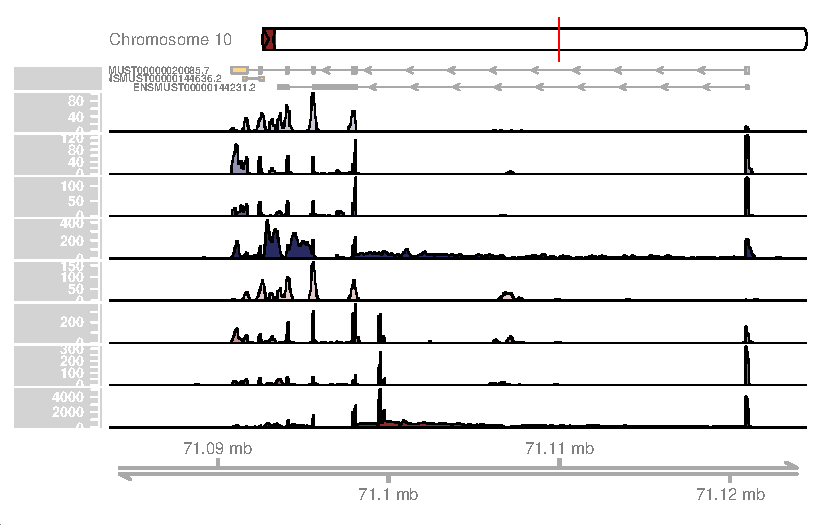
\includegraphics{visualization_bw_files/figure-pdf/test_example-2.pdf}

}

\end{figure}



\end{document}
